\chapter{OVERVIEW}

\section{Background on regex}

Regular expressions (regexes) are an abstraction of keyword search that enables the identification of text using a pattern instead of an exact keyword.


Regexes are commonly used for parsing text using a general purpose language like Python, validating content entered into web forms using Javascript, and searching text files for a particular pattern using tools like grep, vim or Eclipse.



Although regexes are powerful and versatile, they can be hard to understand,  maintain, and debug, resulting in tens of thousands of bug reports~\cite{Spishak:2012:TSR:2318202.2318207}.

Due in part to their common use across programming languages and how susceptible regexes are to error, many researchers and practitioners have developed tools to support more robust regex creation~\cite{Spishak:2012:TSR:2318202.2318207} or to allow visual debugging~\cite{Beck:2014:RVD:2591062.2591111}. Other research has focused on learning regular expressions from  text~\cite{Babbar:2010:CBA:1871840.1871848, Li:2008:REL:1613715.1613719}, avoiding human composition altogether.
Researchers have also explored applying regexes to test case generation~\cite{Ghosh:2013:JAT:2486788.2486925, Galler:2014:STD:2683035.2683100, Anand:2013:OSM:2503903.2503991, Tillmann:2014:TAT:2642937.2642941},
as specifications for string constraint solvers~\cite{Trinh:2014:SSS:2660267.2660372, hampi} and using regexes as queries in a data mining framework~\cite{Begel:2010:CDE:1806799.1806821}.
Regexes are also employed in critical missions like MySQL injection prevention~\cite{Yeole:2011:ADT:1980022.1980229} and network intrusion detection~\cite{network}, or in more diverse applications like DNA sequencing alignment~\cite{1594922}.


Regular expressions are used frequently by developers for many purposes, such as parsing files, validating user input, or querying a database.
Regexes are also employed in MySQL injection prevention~\cite{Yeole:2011:ADT:1980022.1980229} and network intrusion detection~\cite{network}.
However, recent research has suggested that regular expressions (regexes) are hard to understand, hard to compose, and error prone~\cite{Spishak:2012:TSR:2318202.2318207}.
Given the difficulties with working with regular expressions and how often they appear in software projects and processes, it seems fitting that efforts should be made to ease the burden on developers.


\section{Terminology used in this thesis}

To understand how programmers use regular expressions in Python projects, we scraped \dbfetch{nProjScanned} Python projects from GitHub, and recorded regex usages for analysis. Throughout the rest of this paper, we  employ the following terminology:\\

\noindent \textbf{Utilization}: A \emph{utilization} occurs whenever a regex appears in source code.  We detect utilizations by statically analyzing source code and recording calls to the {\tt re} module in Python.
Within a source code file, a {utilization} is composed of a function, a pattern, and 0 or more flags.  Figure~\ref{fig:exampleUsage} presents an example of one regex {utilization}, with key components labeled. The function call is {\tt re.compile}, \verb!(0|-?[1-9][0-9]*)$! is the regex string, or pattern, and {\tt re.MULTILINE} is an (optional) flag. When executed, this {utilization}  will compile a regex object in the variable {\tt r1} from the pattern \verb!(0|-?[1-9][0-9]*)$!, with the \verb!$! token matching at the end of each line because of the {\tt re.MULTILINE} flag. Thought of another way, a regex  utilization is one single invocation of the {\tt re} library.\\

\begin{figure}[tb]
\centering
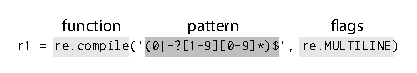
\includegraphics[width=\columnwidth]{nontex/illustrations/exampleUsage.eps}
\vspace{-12pt}
\caption{Example of one regex utilization}
\vspace{-6pt}
\label{fig:exampleUsage}
\end{figure}

\noindent \textbf{Pattern}: A \emph{pattern} is extracted from a utilization, as shown in Figure~\ref{fig:exampleUsage}. In essence, it is a string, but more formally it is an ordered series of regular expression language feature tokens.  The pattern in Figure~\ref{fig:exampleUsage}  will match if it finds a zero at the end of a line, or a (possibly negative) integer at the end of a line (i.e., due to the {\tt -?} sequence denoting zero or one instance of the {\tt -}).

Note that because the vast majority of regex features are shared across most general programming languages (e.g., Java, C, C\#, or Ruby), a Python {pattern} will (almost always) behave the same when used in other languages, whereas a utilization is not universal in the same way (i.e., it may not compile in other languages, even with small modifications to function and flag names).
As an example, the {\tt re.MULTILINE} flag, or similar, is present in Python, Java, and C\#, but  the Python {\tt re.DOTALL} flag is not present in C\# though it has an equivalent flag in Java.

In this work, we primarily focus on patterns since they are cross-cutting across languages and are the primary way of specifying the matching behavior. Next, we describe the research questions, data set collection and analysis.

We consider regex language features to be tokens that specify the matching behavior of a regex pattern, for example,  the {\tt +} in {\tt ab+}.  All studied features are listed and described in Table~\ref{table:featureStats} with examples. We then map the feature coverage for four common regex support tools, brics, hampi, RE2 and Rex, and explore survey responses regarding feature usage for some of the less supported features.\\

\section{Structure of this thesis}
